
\documentclass[a4paper,nobalancelastpage]{revtex4-1}
\usepackage{amsmath,amssymb,graphicx,hyperref,mathtools, color, bm}
\usepackage{sidecap,subcaption}
\usepackage[labelfont=bf]{caption}
\usepackage[labelsep=space]{caption}
\usepackage[font={small}]{caption}
\usepackage{float}

\usepackage{parskip}
\setlength{\parindent}{15pt}
\setlength{\parskip}{8pt}

\graphicspath{{./../figures/weak-coupling/}}

\newcommand{\vect}[1]{\bm{#1}}
% Underlined vector format (bold, single underline)
\newcommand{\uvect}[1]{\bm{\underline{#1}}}
% Underlined matrix format (bold, double underline)
\newcommand{\umat}[1]{\bm{\underline{\underline{#1}}}}
\newcommand{\abs}[1]{\lvert #1 \rvert}
% Automatically expand cos into exponential -- note, pass both arguments positive
\newcommand{\cosexpansion}[2] {\frac{1}{2} \left[ e^{#1} e^{-#2} +e^{-#1}e^{#2} \right]}
\newcommand{\expn}[1] {e^{#1}}
\newcommand{\sinc}[1]{\mathrm{sinc} \ #1}

\begin{document}
\section*{Weak coupling expansion}
\subsection{Perturbatively simplify out light field equation}

Consider light field equation in dimensionless coordinates ($\frac{\sqrt{2} x}{w_z}$), where $w_z$ is the beamwaist at the z-position of the atoms, and $E_0=\mathcal{E}_0 \left( \frac{\sqrt{2}}{w_0}\right)^2$, so that the atomic field and light field are unitless and normalised:

\begin{equation}
\label{eq:eqnalphafirst}
 i\partial_t \alpha_{nm}=(\omega_{n,m}-\omega_{pump}-i\kappa)\alpha_{n,m}+f_{n,m} - E_0 N \sum_{n',m'}  \int \mathrm{d}^2\vect{r} \int \mathrm{d}z |Z(z)|^2 |\psi(\vect{r})|^2 u^*_{m,n}(\vect{r},z) u_{m',n'}(\vect{r},z)\alpha_{m',n'}
\end{equation}

Can rewrite this as:

\begin{equation}
 i\partial_t \alpha_{nm}=-(\Delta_0-i\kappa)\alpha_{n,m}+f_{n,m} - E_0 N \sum_{n',m'} \mathbf{A}_{n,m,n',m'}\alpha_{m',n'}
\end{equation}

where:

\begin{equation}
\label{eq:Amn}
\mathbf{A}_{n,m,n',m'}= \int \mathrm{d}^2 \vect{r} \int  \mathrm{d}z |Z(z)|^2 |\psi(\vect{r})|^2 u^*_{m,n}(\vect{r},z) u_{m',n'}(\vect{r},z)
\end{equation}

We can also write the overall equation for the vector $\uvect{\alpha}$ where $\umat{A}$ is now the matrix given by the overall overlap with the atomic field.

\begin{equation}
i\partial_t \uvect{\alpha} =-(\Delta_0+i\kappa)\uvect{\alpha}- E_0 N \umat{A} \ \uvect{\alpha} + \uvect{f} 
\end{equation}
\\
Need to assume a few things now.
One, that the cavity loss rate $\kappa$ is fast enough that the light reaches a steady state, so that $i \partial_t \uvect{\alpha}=0$ and we can rewrite, factoring $(\Delta_0+i\kappa)$ out of the square bracket:

\begin{equation}
\left[1 + \frac{E_0 N}{(\Delta_0+i\kappa) } \umat{A} \ \right] \ \uvect{\alpha} = \frac{\uvect{f}}{(\Delta_0+i\kappa) }
\end{equation}
\\
Two, that the light and atoms are weakly coupled, i.e. $E_0$ is small compared the other terms in the light equation, and therefore the second term in the square bracket is small, and we can Taylor expand and trucate to get a perturbative expression using $(1-x)^{-1}=\sum_n x^n$ for $\abs{x}<1$.

\begin{align}
\uvect{\alpha} &= \left[1 + \frac{E_0 N}{(\Delta_0+i\kappa) } \umat{A} \ \right]^{-1} \frac{\uvect{f}}{(\Delta_0+i\kappa) }
\\ & = \left[1 - \frac{\mathcal{E}_0 N}{(\Delta_0+i\kappa) } \umat{A} \ +\mathcal{O}^2 \right] \frac{\uvect{f}}{(\Delta_0+i\kappa) } \\ &=
 \frac{\uvect{f}}{(\Delta_0+i\kappa)} -  \frac{E_0 N}{(\Delta_0+i\kappa)^2 } \umat{A} \ \uvect{f}
\end{align}

Or in terms each separate indexed alpha:

\begin{equation}
\alpha_{nm}= \frac{f_{n,m}}{(\Delta_0+i\kappa)} -  \frac{E_0 N}{(\Delta_0+i\kappa)^2 } \sum A_{n,m,n',m'} f_{n',m'}
\end{equation}

\subsection{Substitute in atomic field equation}

We can now consider the (dimensionless) atomic field equation, where we have defined dimensionless quantities in terms of $\omega_z/\sqrt{2}$ as above and in previous notes, and $\eta=\sqrt{2}l_{HO}/\omega_z$ is the ratio of beamwaist to oscillator length (note that $V_{ext}$ will also need to be dimensionless):

\begin{equation}
\label{eq:eqnpsifirst}
i \partial_t \psi(\vect{r})= -\frac{\omega_T \eta^2}{2}\nabla^2 \psi(\vect{r})+ V_{\text{ext}} \psi(\vect{r}) - E_0 
\int \, \mathrm{d}z |Z(z)|^2 \sum_{n,m,n',m'} \alpha_{n,m}^* \ u_{n,m}^* (\vect{r},z)\ \alpha_{n',m'} \ u_{n',m'}(\vect{r},z) \ \psi(\vect{r})
\end{equation}

Substituting in $\alpha_{n,m}$:
  
\begin{align}
i \partial_t \psi(\vect{r})= -& \frac{\omega_T \eta^2}{2}\nabla^2 \psi(\vect{r}) + V_{\text{ext}} \psi(\vect{r}) - E_0 
\int \, \mathrm{d}z |Z(z)|^2 \sum_{n,m,n',m'} u_{n,m}^*(\vect{r},z) u_{n',m'}(\vect{r},z) \nonumber \\ & \left[ \frac{f_{n,m}}{(\Delta_0+i\kappa)} -  \frac{E_0 N}{(\Delta_0+i\kappa)^2 } \sum_{i,j} A_{n,m,i,j} f_{i,j} \right]^*  \left[ \frac{f_{n',m'}}{(\Delta_0+i\kappa)} -  \frac{E_0 N}{(\Delta_0+i\kappa)^2 } \sum_{i',j'} A_{n,m,i',j'} f_{i',j'} \right]  \ \psi(\vect{r})
\end{align}
\\
\subsection{Effective potential term}

There are three terms in this product. The first, the product of the two purely pump-dependent terms, is not evolving -- it's a static pump field which goes to modify the overall external field. We can write:

\begin{equation}
V_{\text{eff}}= V_{\text{ext}} - E_0 
\int \, \mathrm{d}z |Z(z)|^2 \sum_{n,m,n',m'} u_{n,m}^*(\vect{r},z) u_{n',m'}(\vect{r},z) \frac{f_{n,m}}{(\Delta_0-i\kappa)}    \frac{f_{n',m'}}{(\Delta_0+i\kappa)}
\end{equation}

Recalling that in the regime $z_R \gg \sigma_z \gg \lambda$, where $\sigma_z$ is the width of the assumed Gaussian cloud, we can carry out the z-integral:

\begin{align}
\label{eq:z-int}
   O_{n,m,n',m'}(r,z)=\int  dz |Z(z)|^2 
  \cos\left[  f_0(\vect{r},z) - \theta(z) (m+n) \right] & \cos \left[  f_0(\vect{r},z) - \theta(z) (m^\prime+n^\prime) \right] \nonumber \\ &\simeq
  \frac{1}{2}     \cos\left( \theta(z_0) (m+n - m^\prime - n^\prime) \right)
\end{align}
\\
Using 

\begin{equation}
\label{eq:umn}
u_{m,n}(x,y,z) = \chi_n\left( x \right)
  \chi_m\left( y \right)  \cos \left[ f_0(x,y,z) - \theta(z) (m+n) \right]
\end{equation} 

we get:

\begin{align}
\label{eq:Veffinprog}
V_{\text{eff}} (\vect{r}) &= V_{\text{ext}} - E_0 \sum_{n,m,n',m'} \chi_n\left( x \right) \chi_{n'}\left( x \right) 
  \chi_{m'}\left( y \right) 
  \chi_m\left( y \right) \frac{f_{n,m}}{(\Delta_0-i\kappa)}    \frac{f_{n',m'}}{(\Delta_0+i\kappa)}  O_{n,m,n',m'}(\vect{r},z)
\nonumber \\ &= V_{\text{ext}} - \frac{E_0}{2(\Delta_0^2+\kappa^2)} \sum_{n,m,n',m'} f_{n,m} \chi_n\left( x \right)
  \chi_m\left( y \right) f_{n',m'} \chi_{n'}\left( x \right)
  \chi_{m'}\left( y \right) \cos\left( \theta(z_0) (m+n - m^\prime - n^\prime) \right)
\end{align}

\subsection{Interaction term}

This leaves two terms, the sum of the two cross-terms $f * Af$ and the product of the $Af$ terms. 
The latter as is of order $\mathcal{O}(E^3)$ so we drop it in the perturbative approach.
The former, substituting in the expression for $A_{mnm'n'}$ from Eq.\ref{eq:Amn}, yields:

\begin{align}
i \partial_t \psi(\vect{r})=...-
E_0 
\int \, \mathrm{d}z |&Z(z)|^2 \sum_{n,m,n',m'} u_{n,m}^*(\vect{r},z) u_{n',m'}(\vect{r},z) \nonumber \\
&\left[
- \frac{f_{n,m} E_0 N}{(\Delta_0-i\kappa)(\Delta_0+i\kappa)^2} \sum_{i',j'} A_{n',m',i',j'} f_{i',j'} 
- \frac{f_{n',m'} E_0 N}{(\Delta_0+i\kappa)(\Delta_0-i\kappa)^2 } \sum_{i,j} A^*_{n,m,i,j} f^*_{i,j}
\right] 
\end{align}

Now, given that $A_{n,m,n',m'}$, $u_{n,m}(\vect{r},z)$ and $f_{i,j}$ are real, we can drop the complex conjugation:

\begin{align}
i \partial_t \psi(\vect{r})=...-
E_0 
\int \, \mathrm{d}z |&Z(z)|^2 \sum_{n,m,n',m'} u_{n,m} (\vect{r},z) u_{n',m'}(\vect{r},z) \nonumber \\
&\left[
- \frac{f_{n,m} E_0 N}{(\Delta_0-i\kappa)(\Delta_0+i\kappa)^2} \sum_{i',j'} A_{n',m',i',j'} f_{i',j'} 
- \frac{f_{n',m'} E_0 N}{(\Delta_0+i\kappa)(\Delta_0-i\kappa)^2 } \sum_{i,j} A_{n,m,i,j} f_{i,j}
\right] 
\end{align}

From this it's obvious that we can freely relabel the indeces of one of the terms within the square brackets yielding:

\begin{align}
i \partial_t \psi(\vect{r})=&...-
\int \, \mathrm{d}z |Z(z)|^2 \sum_{n,m,n',m'} u_{n,m} (\vect{r},z) u_{n',m'}(\vect{r},z) \nonumber \\
& \qquad f_{n',m'} E^2_0 N  \sum_{i,j} A_{n,m,i,j} f_{i,j}  \left[
- \frac{1}{(\Delta_0-i\kappa)(\Delta_0+i\kappa)^2}
- \frac{1}{(\Delta_0+i\kappa)(\Delta_0-i\kappa)^2 }
\right] \nonumber \\
=&...+ \frac{ 2E^2_0 N \Delta_0 }{(\Delta_0^2+\kappa^2)^2}
\int \, \mathrm{d}z |Z(z)|^2 \sum_{n,m,n',m'} u_{n,m} (\vect{r},z) u_{n',m'}(\vect{r},z) f_{n',m'}  \sum_{i,j} A_{n,m,i,j} f_{i,j}
\end{align}

(note the sign change of the term). Substituting in $A$ from (\ref{eq:Amn}) and $u$ from (\ref{eq:umn}):

\begin{align}
i \partial_t \psi(\vect{r})=&...+ \frac{ 2E^2_0 N \Delta_0 }{(\Delta_0^2+\kappa^2)^2} \sum_{n,m,n',m',i,j}f_{n',m'} f_{i,j}
\chi_n\left( x \right)
  \chi_m\left( y \right) \chi_{n'}\left( x \right)
  \chi_{m'}\left( y \right) \nonumber  \\& \qquad
   \int \, \mathrm{d}z |Z(z)|^2    \cos \left[ f_0(x,y,z) - \theta(z) (m+n) \right]  \cos \left[ f_0(x,y,z) - \theta(z) (m'+n') \right] 
 \nonumber \\ &  \qquad \qquad
  \int \mathrm{d}^2 \vect{r'}  \int  \mathrm{d}z' |Z(z')|^2 |\psi(\vect{r}')|^2 u_{m,n}(\vect{r}',z') u_{i,j}(\vect{r}',z')
  \\ =&
  ...+ \frac{ 2E^2_0 N \Delta_0 }{(\Delta_0^2+\kappa^2)^2} \sum_{n,m,n',m',i,j}f_{n',m'} f_{i,j}
\chi_n\left( x \right)
  \chi_m\left( y \right) \chi_{n'}\left( x \right)
  \chi_{m'}\left( y \right) \nonumber  \\& \qquad
   \frac{1}{2} \cos \left( \theta(z) (m+n-m'-n') \right) \frac{1}{2} \cos \left( \theta(z) (m+n-i-j) \right)  
 \nonumber \\ &  \qquad \qquad
  \int \mathrm{d}^2 \vect{r'}  |\psi(\vect{r}')|^2 \chi_n\left( x' \right) \chi_m\left( y' \right) \chi_i\left( x' \right) \chi_j\left( y' \right)
\end{align}

We can define for convenience an effective interaction $U(\vect{r},\vect{r}')$ such that we may write the interaction term in the form $ \int \mathrm{d}^2 \vect{r'} U(\vect{r},\vect{r}')  |\psi(\vect{r}')|^2  $ -- this means:

\begin{align}
U(\vect{r},\vect{r}')=& \frac{ 2E^2_0 N \Delta_0 }{(\Delta_0^2+\kappa^2)^2} \sum_{n',m'}
 f_{n',m'} \chi_{n'}\left( x \right)
  \chi_{m'}\left( y \right) 
   \sum_{i,j} f_{i,j} \chi_i\left( x' \right) \chi_j\left( y' \right)  
  \nonumber 
\\ 
 &\qquad \sum_{n,m}
  \chi_n\left( x \right)
  \chi_m\left( y \right) 
  \chi_n\left( x' \right) \chi_m\left( y' \right) \nonumber 
\\ 
 &\qquad \qquad \frac{1}{2} \cos \left( \theta(z) (m+n-m'-n') \right) \frac{1}{2}    
 \cos \left( \theta(z) (m+n-i-j) \right)    \nonumber 
\\ 
=& \frac{ 2E^2_0 N \Delta_0 }{4(\Delta_0^2+\kappa^2)^2} \sum_{n',m'}
 f_{n',m'} \chi_{n'}\left( x \right)
  \chi_{m'}\left( y \right) 
   \sum_{i,j} f_{i,j} \chi_i\left( x' \right) \chi_j\left( y' \right)  
 \nonumber 
\\ 
 & \qquad \sum_{n,m}
\chi_n\left( x \right)
  \chi_m\left( y \right) 
  \chi_n\left( x' \right) \chi_m\left( y' \right) 
\cosexpansion{\theta_z(n+m)}{\theta_z(n'+m')}
 \nonumber 
\\
& \qquad \qquad \cosexpansion{\theta_z(n+m)}{\theta_z(i+j)} \nonumber 
\\
=&\frac{ 2E^2_0 N \Delta_0 }{4(\Delta_0^2+\kappa^2)^2} \sum_{n',m'}
 f_{n',m'} \chi_{n'}\left( x \right)
  \chi_{m'}\left( y \right) 
   \sum_{i,j} f_{i,j} \chi_i\left( x' \right) \chi_j\left( y' \right)  
   \nonumber 
\\
& \qquad \sum_{n,m}
\chi_n\left( x \right)
  \chi_m\left( y \right) 
  \chi_n\left( x' \right) \chi_m\left( y' \right)  \nonumber 
\\ 
& \qquad \quad \big[
   \expn{\theta_z (2(n+m)-i-j-n'-m')} +
   \expn{\theta_z (n'+m'-i-j)}   +
   \expn{\theta_z (i+j-n'-m')} +
   \expn{\theta_z (i+j+n'+m'-2(n+m))}
  \big]
\end{align}

\subsection{Define pump and kernel functions}

We can tidy this up by defining a complex pump term a complex integral kernel $D(\vect{r},\vect{r}',\xi)$:

\begin{equation}
D(\vect{r},\vect{r}',\xi)= \sum_{n,m} \chi_{n}\left( x \right)
  \chi_{m}\left( y \right) \chi_{n}\left( x' \right)
  \chi_{m}\left( y' \right)  \expn{-i \xi (m+n)}
\end{equation}

and a complex pump term $F(\vect{r},\xi)$:

\begin{equation}
F(\vect{r},\xi)= \sum_{n,m} f_{n,m} \chi_{n}\left( x \right)
  \chi_{m}\left( y \right) \expn{-i \xi (m+n)}
\end{equation}

Recalling that $f_{nm}=\int d\vect{r} f(\vect{r}) u_{m,n}(\vect{r},-z_R)$ we can write this as:

\begin{equation}
F(\vect{r},\xi)= \sum_{n,m} \int d\vect{r}' f(\vect{r}) \chi_{n}\left( x' \right)
  \chi_{m}\left( y' \right) \chi_{n}\left( x \right)
  \chi_{m}\left( y \right) \expn{-i \xi (m+n)}
\end{equation}

Note that the $\xi$ term in this can be complex, the real part of this is the Guoy phase, and any complex part to it is equivalent to imposing a cutoff in the modes we're considering. To keep the first 20 modes for example, we can set $\xi=\theta(z_0)+i \gamma$, where $\gamma=\frac{1}{number \ of \ modes}$.

[Note also that the cos term is one, as seen by substituting in coordinated on mirror $-z_M+\frac{r^2}{2|R_M|}$, $R(-z_M)=-|R_M|$, $\psi(z_M)=\pi/4$ and obtaining an expression for $\xi_{q_0}$ from Gaussian optics crib notes, which cancels all other terms.]
\\
This is clearly related to the integral kerel:

\begin{equation}
F(\vect{r},\xi)= \int d\vect{r}' f(\vect{r}') D(\vect{r},\vect{r}',\xi)
\end{equation}

Consider now the kernel term -- it appears everywhere, so doing something contructive with it would be good. By using Mehler's kernel we can rewrite the oscillator Green's function. 

We define the function:

\begin{equation}
\label{eq:kernInChis}
K(x,x',\xi)=\sum_{n} \chi_n (x) \chi_n (x') e^{i\xi n}
\end{equation}

which by using Mehler's Kernel

\begin{equation}
\sum_{n}^{\infty} \frac{(\rho/2)^n}{n!} H_n(x) H_n(x') = \frac{1}{\sqrt{1-\rho^2}}
\exp{\left(-
\frac{\rho^2(x^2+x'^2)-2\rho x x'}{(1-\rho^2)}\right)
}
\end{equation}

we can rewrite explicitly in real space:

\begin{equation}
\label{eq:integralkernelK}
K(x,x',\xi)=\sqrt{\frac{e^{\xi}}{i \pi \sin(\xi)}} \exp{\left[ 
\frac{i }{2 } \left(
\frac{x^2+x'^2}{\tan(\xi)}-\frac{2 x x'}{\sin(\xi)}
\right) \right] }
\end{equation}

To obtain the proper symmetry, i.e. keep only even order modes, our integral kernel $D$ then needs to include a factor of $\frac{1}{2}[(1-(1)^(n+m))]$, i.e. the full kernel should read:

\begin{equation}
D(\textbf{r},\textbf{r}',\xi)= \sum_{n,m} \frac{1}{2} (1+(-1)^{n+m}) \chi_n (x) \chi_n (x') \chi_m (y) \chi_m (y') e^{i\xi(n+m)}
\end{equation}

The $(-1)^n$ term yields a sign change in the $xx'$ term, i.e.:

\begin{equation}
\sum_{n} (-1)^n \chi_n (x) \chi_n (x') e^{i\xi n}= \sqrt{\frac{e^{\xi}}{i \pi \sin(\xi)}} \exp{\left[ \frac{i }{2 } \left(
\frac{x^2+x'^2}{\tan(\xi)}+\frac{2 x x'}{\sin(\xi)}  
\right) \right] } =
K(x,-x',\xi)
\end{equation}

So the kernel with the correct parity will read:

\begin{equation}
\label{eq:integralkernelD}
D(\textbf{r},\textbf{r}',\xi)=\frac{1}{2} \big[ K(x,x',\xi)K(y,y',\xi)+ K(x,-x',\xi)K(y,-y',\xi) \big]
\end{equation}

\subsection{Finalised terms and equation of motion}

We define $\theta(z_0)=\theta_0$ for convenience. This is the Gouy phase at the z-position of the atoms.
We can rewrite the effective potential in terms of these pump and kernel terms with a mode cutoff for completeness, expanding the cos in (\ref{eq:Veffinprog}), and noting $F(\vect{r},\theta(z_0))^*=F(\vect{r},-\theta(z_0))$:

\begin{align}
\label{eq:Veff}
V_{\text{eff}} (\vect{r}) = V_{\text{ext}} - \frac{E_0}{2(\Delta_0^2+\kappa^2)} \abs{F(\vect{r},\theta_0+i \gamma)}^2
\end{align}

And the $U(\vect{r},\vect{r}')$ (without mode cutoff) reads (including the parity considerations above):

\begin{align}
\label{eq:Urr}
U(\vect{r},\vect{r}')=&\frac{ 2E^2_0 N \Delta_0 }{4(\Delta_0^2+\kappa^2)^2} 
\bigg[
F(\vect{r},-\theta_0)F(\vect{r}',-\theta_0)D(\vect{r},\vect{r}',2\theta_0) 
+ F(\vect{r},\theta_0)F(\vect{r}',\theta_0)D(\vect{r},\vect{r}',-2\theta_0) +\nonumber \\ &  \qquad \qquad 
F(\vect{r},\theta_0)F(\vect{r}',-\theta_0)D(\vect{r},\vect{r}',0)
+ F(\vect{r},-\theta_0)F(\vect{r}',\theta_0)D(\vect{r},\vect{r}',0)
\bigg]
\end{align}

and we just add $+i\gamma$ to each $\xi$ argument for mode cutoffs.

The full equation of motion is:

\begin{equation}
i \partial_t \psi(\vect{r})= \bigg( 
\frac{\eta^2 \omega_T}{2}\nabla^2 \psi(\vect{r}) + V_{\text{eff}} (\vect{r}) \ \psi(\vect{r})+\int \mathrm{d} \vect{r}' U(\vect{r},\vect{r}') \abs{\psi(\vect{r}')}^2
\bigg) \psi(\vect{r})
\end{equation}

with $U(\vect{r},\vect{r}')$ as in Eq. \ref{eq:Urr} and $V_{\text{eff}}(\vect{r})$ from Eq. \ref{eq:Veff}.

\subsection{Calculating $F(r,\xi)$ with Gaussian pump spot}

Assuming a Gaussian pump $f(\vect{r})=f_0 \exp{(-\vect{r}^2/2\sigma_P^2)}$ we can rewrite $F(\textbf{r},\xi)$ as:

\begin{equation}
F(\textbf{r},\xi)=\frac{f_0}{2} \bigg[ 
\phi(x,\xi)\phi(y,\xi)+\phi(-x,\xi)\phi(-y,\xi)
\bigg]
\end{equation}

where we define $\phi(x,\xi)$ as:

\begin{equation}
\phi(x,\xi)=\int dx' e^{-\frac{x'^2}{2 \sigma_P^2}} K(x,x',\xi)
\end{equation}

with the 1D kernels $K(x,x',\xi)$ from Eq.\ref{eq:integralkernelK}. This can be computed directly:

\begin{align}
\phi(x,\xi) &=\frac{e^{\xi}\exp{\left(\frac{i x^2}{2 \tan(\xi)} \right) }}
{\sqrt{i \pi \sin(\xi)}}  \int dx' \exp{\left[ 
\left( \frac{x'^2}{2 \sigma_P^2}-\frac{i }{2 \tan(\xi)} 
\right) x'^2
-\frac{2 x }{\sin(\xi)}x'
\right] } \nonumber \\
&=
\sqrt{\frac{2 e^{\xi}}{i \sin(\xi) \left( \frac{1}{\sigma_P^2}-\frac{i}{\tan(\xi)} \right)}}
\exp{\left[ -\frac{x^2}{2} \left( \frac{1+i \sigma_P^2 \tan(\xi)}{\sigma_P^2+i \tan(\xi)}  \right) \right]}
\end{align}

Tidying this up slightly:

\begin{equation}
\phi(x,\xi) =
\sqrt{
\frac{2 \sigma_P^2 e^{\xi}}{\sigma_P^2\cos(\xi)+i \sin(\xi)} 
}
\exp{
\left[ 
-\frac{x^2}{2} \left( \frac{\cos(\xi)+i \sigma_P^2 \sin(\xi)}{\sigma_P^2 \cos(\xi)+i  \sin(\xi)}  \right) 
\right]
}
\end{equation}

This only depends on $x^2$ so the two components of $F(\textbf{r},\xi)$ will be the same, and we can easily write:

\begin{equation}
F(\textbf{r},\xi)=
\frac{2 \sigma_P^2 f_0 e^{\xi}}{\sigma_P^2\cos(\xi)+i \sin(\xi)} 
\exp{
\left[ 
-\frac{\vect{r}^2}{2} \left( \frac{\cos(\xi)+i \sigma_P^2 \sin(\xi)}{\sigma_P^2 \cos(\xi)+i  \sin(\xi)}  \right) 
\right]
}
\end{equation}

Two limiting cases of this are a very large pump spot, and a very narrow pump spot.\\
\\
In the case of a wide pump spot, i.e. $\sigma_P$ much bigger than all other quantities involved, we have:

\begin{equation}
F(\textbf{r},\xi)=
\frac{2 f_0 }{\cos(\xi)} 
\exp{
\left[ \xi
-i \frac{\vect{r}^2}{2} \tan{\xi}
\right]
}
\end{equation}

whereas for a small spot size we get:

\begin{equation}
F(\textbf{r},\xi)=
\frac{2 \sigma_P^2 f_0 }{i \sin(\xi)} 
\exp{
\left[ \xi
-\frac{\vect{r}^2}{2 i \tan \xi} 
\right]
}
\end{equation}

remembering that $\xi=\theta(z)-i \alpha$, where alpha is the mode cutoff ($\alpha=0$ is keeping all modes).



\begin{center}
 \begin{tabular}{|c | c | c|} 
 \hline
$\theta_z=0$ 
& $\tan{\theta_z} \rightarrow 0$ 
& $F_{wide}(\textbf{r},\theta_z)\rightarrow 0$ 
\\ 
& $\cot{\theta_z} \rightarrow \infty$  
& $F_{narrow}(\textbf{r},\theta_z)\rightarrow \infty$ 
\\
& $\cos{\theta_z} \neq 0$  
& 
\\
& $\sin{\theta_z} = 0 $ 
& 
\\
\hline
$\theta_z=\pi / 4$ 
& $\tan{\theta_z} = \cot{\theta_z}$ 
& $F_{narrow}(\textbf{r},\theta_z)=F_{wide}^*(\textbf{r},\theta_z) $ 
\\
& $\cos{\theta_z} = \sin{\theta_z}$  
& 
\\
\hline
$\theta_z=\pi / 2 $
& $\tan{\theta_z} \rightarrow \infty $
& $F_{wide}(\textbf{r},\theta_z)\rightarrow \infty $
\\ 
& $\cot{\theta_z} \rightarrow 0  $
& $F_{narrow}(\textbf{r},\theta_z)\neq 0 $
\\
 & $\cos{\theta_z} \neq 0  $
 & 
 \\
 & $\sin{\theta_z} = 0  $
 & 
 \\
\hline
\end{tabular}

\end{center}

\subsection{Concerning the delta-function like behaviour of $D(r,r',\xi)$ at $\xi=0$}

Two ways to convince yourself it's a delta function

\begin{itemize}
\item we know this is the Green's function of HO, and for this reason we know that after one period the oscillator returns to itself (with an overall phase factor of +-1) i.e. same eigenstates 
\item a delta function is something that (a) integrates to one and (b) integrated over with another function, it yields the function at the point of the delta function. If we take D, we can convince ourselves that the contributions from r=/=rp are either fast-oscillating, or cancel, i.e. only the r=rp contributes to this.
\end{itemize}

We need to code Eq.\ref{eq:Urr}, which contains some of these $D(r,r',0)$ terms, in the interaction term 

\begin{equation}
U^{int}=\int \mathrm{d} \vect{r}' U(\vect{r},\vect{r}') \abs{\psi(\vect{r}')}^2
\end{equation}

 We can write this integral as having a "regular" part, i.e. the contributions from the $2\theta_0$ terms which are well behaved everywhere but at the ends of the cavity (which we expect), and a part involving the terms which yield deltas, something like:

\begin{equation}
U^{int}=\int \mathrm{d} \vect{r}' U^{reg}(r,r')|\psi(\vect{r}')|^2 +\int \mathrm{d} \vect{r}' U^{delta}(r,r') \abs{\psi(\vect{r}')}^2
\end{equation}

where

\begin{align}
U^{reg}(\vect{r},\vect{r}')=&\frac{ E^2_0 N \Delta_0 }{2(\Delta_0^2+\kappa^2)^2} 
\bigg[
F(\vect{r},-\theta_0)F(\vect{r}',-\theta_0)D(\vect{r},\vect{r}',2\theta_0) 
+ F(\vect{r},\theta_0)F(\vect{r}',\theta_0)D(\vect{r},\vect{r}',-2\theta_0) \nonumber 
\bigg]
\end{align}

and 

\begin{align}
U^{delta}(\vect{r},\vect{r}')=\frac{ E^2_0 N \Delta_0 }{2(\Delta_0^2+\kappa^2)^2} 
\bigg[&
F(\vect{r},\theta_0)F(\vect{r}',-\theta_0)
\big(\delta(r-r')+\delta(r+r') \big)
\\&+ F(\vect{r},-\theta_0)F(\vect{r}',\theta_0) \big(\delta(r-r')+\delta(r+r') \big) \nonumber 
\bigg]
\end{align}

but since $F$ only depends on $r^2$, so the $\pm r$ delta functions just contribute a factor of 2.

We can code the integral of $U^{reg}$ as is, and we can carry out the integral of the delta functions explicitly, to get:


\begin{align}
\label{eq:Utot}
U^{tot}=
\int \mathrm{d} \vect{r}' U^{reg}(r,r')|\psi(\vect{r}')|^2 +\frac{ E^2_0 N \Delta_0 }{(\Delta_0^2+\kappa^2)^2} 
\bigg[&
F(\vect{r},\theta_0)F(\vect{r},-\theta_0)+ F(\vect{r},-\theta_0)F(\vect{r},\theta_0) \nonumber 
\bigg]|\psi(\vect{r})|^2
\end{align}

\subsection{Comparing weak coupling code results to notes (extracting wavevector)}

We have a semiperiodic output from the code for negative delta which suggests the system does go unstable. We want to extract the k vectors from this oscillation so that they can be compared.

\begin{figure}[H]
  \centering
  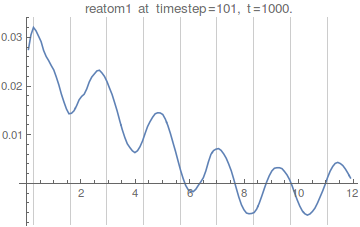
\includegraphics[width=3in]{FToriginaldata}
  \caption{Original output of the real part of the atomic field (reatom1 from the Mathematica notebook) at timestep indicated, with gridlines to show periodicity or lackthereof.}
\end{figure}

In general terms, what we do have is some function $f(x)$, which is really in discrete intervals, i.e. it is really $f_n$, the function at position $x_n$, where $x_n=n \Delta x$, $n=0...(N-1)$, where N is the number of points in our grid from the code, and $\Delta x$ is the grid spacing. Note that the sum goes from $[0,N-1]$ instead of $[1,N]$ like in the code.

We want the Fourier transform $\tilde{f}(k)=\int dx f(x) e^{i k x}$, but given that this is really a discrete function, we need to write:

\begin{equation}
\tilde{f}(k)=\sum_{n=0}^{N-1}\Delta x f_n e^{i k n\Delta x}
\end{equation}

We can generate a FT in Mathematica using the Fourier command. For this we need to 'lose' the x axis information and only plot the y values against integers, which means we will then need to re-define the interval between the plotted k-space points to match our original real space range.

\begin{figure}[H]
\begin{subfigure}{.5\textwidth}
  \centering
  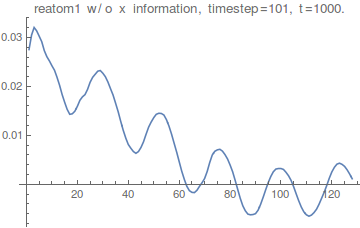
\includegraphics[width=3in]{FTdimensionlessdata}
	\subcaption{}  
\end{subfigure}
\begin{subfigure}{.5\textwidth}
\centering
   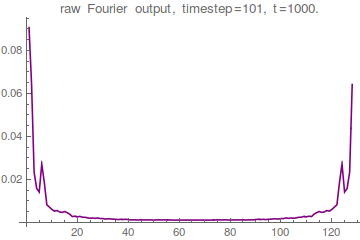
\includegraphics[width=3in]{FTunmanipulatedtransf}
   	\subcaption{}  
\end{subfigure}
\caption{'Flattened' data containing just the y-values (a), and the result of just putting it through the Fourier[] Mathematica function (b).}
\end{figure}

Firs of all, from the Mathematica documentation, we can see the Fourier function uses the definition (adjusting indeces and matching symbols to our problem):

\begin{equation}
\mathcal{F}(f_n)=
\frac{1}{\sqrt{N}} \sum_{n=0}^{N-1} f_n e^{i 2 \pi n s/N}
\end{equation}

where s is the k-space index.

This means that $2 \pi n s/N$ is the equivalent of $k n \Delta x$, therefore we have:

\begin{equation}
\label{eq:FTkcorrected}
k_s=\frac{2 \pi s}{N \Delta x}
\end{equation}

and also taking care of prefactors, defining $\tilde{f}_s$ as the discrete FT in k-space just as we defined $f_n$ in real space, we get:

\begin{equation}
\tilde{f}_s=\Delta x \sqrt{N} \mathcal{F}(f_n)
\end{equation}

i.e. we now have the correct pre-factors compared to the code output, and the correct renormalisation of the x-axis in k space, to fix Fig (2.a).

We now need to consider the aliasing that we see in the original output of the Fourier Mathematica function Fig. (2.b), i.e. the high s contributions that are actually due to negative wavevector of the symmetric k-space distribution. To understand this, consider the negative k contributions:

\begin{equation}
\tilde{f}(-k)=\sum_{n=0}^{N-1} \Delta x f_n e^{-in\Delta x k}
\end{equation}

We can always multiply this by $e^{i 2 \pi m}$, where m is any integer (we are then free to make it correspond to n); doing this, and replacing in the expression for k Eq.\ref{eq:FTkcorrected}, yields:

\begin{equation}
\tilde{f}(-k)=\sum_{n=0}^{N-1} \Delta x f_n e^{-i n 2 \pi s/N}e^{i 2 \pi n}=\sum_{n=0}^{N-1} \Delta x f_n e^{i 2\pi (N-s)/N }
\end{equation}

i.e. we get that $f_{-s}=f_{N-s}$, which is what we see in Fig.(2.b).

To correct both the aliasing and the redimensioning of the x-axis, we need to apply both considerations: Eq.\ref{eq:FTkcorrected} to generate x-values, and moving the tail of Fig.(2.b) to the correct negative values. 

\begin{figure}[H]
  \centering
  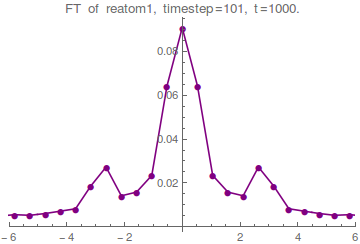
\includegraphics[width=3in]{FTfinished}
  \caption{Fourier transform of the real part of the atomic field at time indicated.}
\end{figure}

We can sanity check this result by a few observations.

Firstly, we see a $\sinc{x}=(\sin x)/x$ envelope on the FT spectrum. This is due to the finite range in x of the original data. Consider this: when we set up the FT integral on a finite range, what we're really doing is convolving it with a step function $\Theta(x_{max}-x)$, which makes the integral zero beyond $x>x_{max}$. (Actually going to do this as if symmetric function because it's just easier to compare to sinc).

\begin{equation}
\int dx f(x) e^{ikx} \Theta(x_{max}-x)
\end{equation}

?

\begin{equation}
\int_{-a}^{a} e^{ikx} dx = 2 a \ \sinc{(ka)}
\end{equation}

Secondly, note that we see five data points in k-space to the first maximum. This makes sense if we look at the original data: we can see there's roughly five periods in the range we have, which means $x_{period}\approx x_{tot}/5$. This means $k_{period}=2 \pi/ x_{period}=5 \times(2 \pi /x_{tot})$ which using Eq.\ref{eq:FTkcorrected} gives us $s=5$. 

Furthermore, from Eq.\ref{eq:FTkcorrected} we can see that to get a higher resolution in k-space, we don't need a finer grid in real space, but a larger x range $x_{tot}$.

\subsection{Long range and short range components of the interaction term $U(r,r')$}

We have calculated the total interaction term in Eq.\ref{eq:Utot}, observing that this has a 'regular' contribution and a delta function contribution. To rephrase this into a more physically relevant observation, we can observe this has a \textbf{short-range} interaction part, given by the delta function terms which are local, and a \textbf{long-range} interaction part, given by the remaining terms, i.e.:

\begin{equation}
U^{tot}(r,r')=U^{short}(r)+U^{long}(r,r')
\end{equation}

with:

\begin{equation}
U^{short}(r)=\frac{ 2 E^2_0 N \Delta_0 }{(\Delta_0^2+\kappa^2)^2}
F(\vect{r},\theta_0)F(\vect{r},-\theta_0)|\psi(\vect{r})|^2
\end{equation}

and:

\begin{align}
U^{long}(\vect{r},\vect{r}')=&\int d \vect{r}' \frac{ E^2_0 N \Delta_0 }{2(\Delta_0^2+\kappa^2)^2} 
\bigg[
F(\vect{r},-\theta_0)F(\vect{r}',-\theta_0)D(\vect{r},\vect{r}',2\theta_0) 
+ F(\vect{r},\theta_0)F(\vect{r}',\theta_0)D(\vect{r},\vect{r}',-2\theta_0) \nonumber 
\bigg] \abs{\psi(\vect{r}')}^2
\end{align}

We can go ahead and compute this into something manageable. Taking a large Gaussian pump spot, Eq.\ref{}, for the first of the components of $U^{long}$ we get:

\begin{align}
F(\vect{r},-\theta_0)F(\vect{r}',-\theta_0)D(\vect{r},\vect{r}',2\theta_0) =\left(\frac{2 f_P}{\cos \theta_0}\right)^2 \frac{1}{2 \pi i \sin 2\theta_0}
\exp &\left[\frac{i}{2}(\vect{r}^2+\vect{r}'^2) \left( \tan \theta_0 + \frac{1}{ \tan 2\theta_0} \right) \right] 
\nonumber
\\
 &\times \left[ \exp\left(\frac{i \vect{r}\vect{r}'}{\sin 2\theta_0} \right) + \exp\left(-\frac{i \vect{r}\vect{r}'}{\sin 2\theta_0} \right) \right]
\end{align}

Using the fact that $\tan x + \frac{1}{ \tan 2x} = \frac{1}{ \sin 2x}$, we get:

\begin{align}
F(\vect{r},-\theta_0)F(\vect{r}',-\theta_0)D(\vect{r},\vect{r}',2\theta_0) =\left(\frac{2 f_P}{\cos \theta_0}\right)^2 \frac{1}{2 \pi i \sin 2\theta_0} \left[
 \exp\left(\frac{i (\vect{r}+\vect{r}')^2} {2 \sin 2\theta_0} \right) + \exp\left(\frac{i (\vect{r}-\vect{r}')^2}{2 \sin 2\theta_0} \right) \right]
\end{align}

Similarly for the second term (notice the minus sign):

\begin{align}
F(\vect{r},\theta_0)F(\vect{r}',\theta_0)D(\vect{r},\vect{r}',-2\theta_0) =\left(\frac{2 f_P}{\cos \theta_0}\right)^2 \frac{-1}{2 \pi i \sin 2\theta_0} \left[
 \exp\left(-\frac{i (\vect{r}+\vect{r}')^2} {2 \sin 2\theta_0} \right) + \exp\left(-\frac{i (\vect{r}-\vect{r}')^2}{2 \sin 2\theta_0} \right) \right]
\end{align}

Combining $\frac{1}{2 i}\left[\exp\left(\frac{i (\vect{r}-\vect{r}')^2}{2 \sin 2\theta_0} \right) - \exp\left(-\frac{i (\vect{r}-\vect{r}')^2}{2 \sin 2\theta_0} \right)  \right]$ into $\sin \left( \frac{(\vect{r}-\vect{r}')^2}{2 \sin 2\theta_0} \right)$

and likewise for $\abs{r+r'}$ terms, we get:

\begin{align}
U^{long}(\vect{r},\vect{r}')=& 
\frac{ f_P^2 E^2_0 N \Delta_0 }{\pi (\Delta_0^2+\kappa^2)^2}  \frac{1}{\cos^2 \theta_0 \sin 2\theta_0}
\int d \vect{r}' \bigg[ \sin{\left( \frac{\abs{\vect{r}+\vect{r}'}^2}{2 \sin 2\theta_0} \right)} + \sin{\left( \frac{\abs{\vect{r}-\vect{r}'}^2}{2 \sin 2\theta_0} \right)} \bigg] \abs{\psi(\vect{r}')}^2
\end{align}

\subsection{Discussion of results so far}

\end{document}